%%%%%%%%%%%%%%%%%%%%%%%%%%%%%%%%%%%%%%%%%%%%%%%%%%%%%%%%%%%%%%%%%%%%%%%%%%%%%%%%
% Power Settings
%%%%%%%%%%%%%%%%%%%%%%%%%%%%%%%%%%%%%%%%%%%%%%%%%%%%%%%%%%%%%%%%%%%%%%%%%%%%%%%%
\chapter{Power Settings} \label{Power Settings}
\vspace{-10ex}\mPS{syml}\vskip 8ex

%%%%%%%%%%%%%%%%%%%%%%%%%%%%%%%%%%%%%%%%%%%%%%%%%%%%%%%%%%%%%%%%%%%%%%%%%%%%%%%%
% Introduction
%%%%%%%%%%%%%%%%%%%%%%%%%%%%%%%%%%%%%%%%%%%%%%%%%%%%%%%%%%%%%%%%%%%%%%%%%%%%%%%%
\section{Introduction}

Allows configuring timers for putting the device into \sPoNa{f} or \sPoSl{f}
states and auto-stopping the \mAu{f}.  Also allows for configuring an amount of
time in seconds that can be used to force the device into a \sPoSl{f} state
using \aTo{f}.

\par\medskip

As a semi-portable device that can run on the \cRB{f}, these settings can be
used to prolong the battery charge.  See \hyperref[Power]{\mPo{f}} for
information on the different power states and what they do.

\par\medskip

There are a few ways to get to \mPS{f} depending on which direction the
\cRs{f} is pointing and which mode the device is currently in.  The most
straightforward way is:

\begin{enumerate}
  \item \aTu{f} the \cRs{f} to the \dRi{f}.
  \item \aPH{f} the \cEs{f} until \symD{====} is blinking on the \cDi{f} then
    \aRe{f}.
\end{enumerate}

\begin{table}[H]
\ers{2.0}
\centering
\begin{tabu} { X[1,c,m] | X[1,c,m] | X[1,c,m] }
  \thrule
  \thbi{Position} & \thbi{Mode} & \thbi{Action} \\ \thrule

  \sMi & \multirow{2}{*}[-1mm]{\mode{s}{ANY}}
    & $\hskip 3mm$ \sMtoR \\ \dcrule{1}{1} \dcrule{3}{3}
  \sLe & & \sLtoR \\ \mdrule

  \multirow{4}{*}[-1.5mm]{\sRi} & \mTi{sym} & \sSec \\ \dcrule{2}{3}
    & \multirow{2}{*}[-1mm]{\mSN{sym}} & \sSec \quad \sSec \\ \dcrule{3}{3}
    & & \sTer \quad \sSec \\ \dcrule{2}{3}
    & \state{f}{ANY} & \sRtoM \quad\quad \sMtoR \quad\quad \sSec \\

  \bhrule
\end{tabu}
\caption{Power Settings - Mode}
\end{table}

A few items of note:

\begin{itemize}
  \item The values initially loaded will be the last saved values.
  \item Until a setting has been saved, current \mPo{f} settings will be
    in effect.  That is, the device may \sPoNa{f} or \sPoSl{f} while in
    \mPS{f} mode, but will only do so if left idle.
  \item To \aReset{f} and start over, \aPH{f} the \cEs{f} until you see
        \symD{<<<<} blink on the \cDi{f}.
\end{itemize}

%%%%%%%%%%%%%%%%%%%%%%%%%%%%%%%%%%%%%%%%%%%%%%%%%%%%%%%%%%%%%%%%%%%%%%%%%%%%%%%%
% Overview
%%%%%%%%%%%%%%%%%%%%%%%%%%%%%%%%%%%%%%%%%%%%%%%%%%%%%%%%%%%%%%%%%%%%%%%%%%%%%%%%
\section{Overview}

There are a number of states \mTi{f} can be in and are explained in the next
sections.

\ers{1}
\begin{table}[H]
\centering
\begin{tabu} { X[1,c,m] | X[3,l,m] }
  \thrule
  \thbi{State} & \thbi{Description} \\ \mrule

  \sPSMe{sym} & Select a power setting option. \\ \drule{2}
  \sPSHM{sym} & Set the \textit{hours} or \textit{minutes}
    of the setting selected. \\ \drule{2}
  \sPSMS{sym} & Set the \textit{minutes} or \textit{seconds}
    of the setting selected. \\ \drule{2}
  \sPSSe{sym} & Set the seconds for \textit{touch} induced sleep. \\ \drule{2}
  \sPSDo{sym} & Display setting. \\
  \bhrule
\end{tabu}
\caption{Power Settings - States}
\end{table}

The \sPSMe{f} has \num{4} options to select from:

\begin{table}[H]
\ers{0.1}
\centering
\begin{tabu}{c c}
  \thi{Option} & \thi{Display} \\ \mrule
  \mPSNa{sym} & \symD{nAP!} \\
  \mPSSt{sym} & \symD{StOP} \\
  \mPSSl{sym} & \symD{SLEE.} \\
  \mPSTo{sym} & \symD{tUCH} \\
\end{tabu}
\end{table}

The general progression involves first selecting a menu option, then
setting the timer for that option.  \aTu{f} the \cEs{f} to cycle through the
menu options, \aPR{f} the \cEs{f} to select one, then proceed to set the timer
for that option.

\ase{1}{{c c l c c c c c c c c}}{%
\multirow{4}{*}{\sPSMe{sym}} & \multirow{4}{*}{\sTu}
  & \eSel{sym}{} \mPSNa{sym} & & & & & & & & \\ \dcrule{3}{3}
& & \eSel{sym}{} \mPSSt{sym} & \sPR & \sPSHM{sym} & \sTu & \sPR
  & \sPSMS{sym} & \sTu & \sPR & \sPSDo{sym} \\ \dcrule{3}{3}
& & \eSel{sym}{} \mPSSl{sym} & & & & & & & & \\ \dcrule{3}{11}
& & \eSel{sym}{} \mPSTo{sym} & \sPR & \sPSSe{sym}
  & \sTu & \sPR & \sPSDo{sym} & & & \\}

%%%%%%%%%%%%%%%%%%%%%%%%%%%%%%%%%%%%%%%%%%%%%%%%%%%%%%%%%%%%%%%%%%%%%%%%%%%%%%%%
% Menu
%%%%%%%%%%%%%%%%%%%%%%%%%%%%%%%%%%%%%%%%%%%%%%%%%%%%%%%%%%%%%%%%%%%%%%%%%%%%%%%%
\section{Menu} \sPSMe{syml}

Select a power setting to configure.

\par\medskip

The \sPSMe{f} is where you will select the power setting you want to configure a
timer for.  There are \num{4} options to select from.

\begin{table}[H]
\ers{3}
\begin{tabu}{ X[1,c,m] | X[1,c,m] }
  \thrule
  \thbi{Option} & \thbi{Display} \\ \mrule
  \mPSNa{sym} & \sDl{nAP!} \\ \drule{2}
  \mPSSt{sym} & \sDl{StOP} \\ \drule{2}
  \mPSSl{sym} & \sDl{SLEE.} \\ \drule{2}
  \mPSTo{sym} & \sDl{tUCH} \\
  \bhrule
\end{tabu}
\end{table}

\par\medskip

\mPSNa{f}, \mPSSt{f} and \mPSSl{f} can be set from \num{10} seconds
to \num{99} hours and \num{99} minutes.  Setting the timer to \symD{!0:00}
disables the setting.  If you roll over into hours a \textit{decimal} at the
\textit{bottom right} of the \cDi{f} is used to indicate that the time is in
hours and minutes or \mono{HH:MM} format.

\begin{table}[H]
\centering
\ers{0.1}
\begin{tabu}{c c c c c}
  \sDl{!0:00} & \sDl{!0:10} & \sDl{59:00} & \sDl{!1:00.} & \sDl{99:99.} \\
  \rowfont{\scriptsize} Disabled & Minimum Time & 59 Minutes & 1 Hour & Maximum Time
\end{tabu}
\end{table}

\mPSTo{f} can be set from \num{2} to \num{60} seconds.  Setting the seconds
to \symD{!!!0} disables the setting.

\begin{table}[H]
\centering
\ers{0.1}
\begin{tabu}{c c c}
  \sDl{!!!0} & \sDl{!!!2} & \sDl{!!60} \\
  \rowfont{\scriptsize} Disabled & Minimum Seconds & Maximum Seconds
\end{tabu}
\end{table}

To select an option, \aTu{f} the \cEs{f} then \aPR{f}.

\as{{c c c}}{\multirow{2}{*}{\sPSMe{sym}} & \sTu & \sPR \\
  & \eUp{sym}{MENU OPTION} & \eSel{sym}{MENU OPTION} \\}

%%%%%%%%%%%%%%%%%%%%%%%%%%%%%%%%%%%%%%%%%%%%%%%%%%%%%%%%%%%%%%%%%%%%%%%%%%%%%%%%
% Menu - Nap
%%%%%%%%%%%%%%%%%%%%%%%%%%%%%%%%%%%%%%%%%%%%%%%%%%%%%%%%%%%%%%%%%%%%%%%%%%%%%%%%
\subsection{Nap} \mPSNa{syml}

Set the amount of idle time that needs to pass before the device enters a
\sPoNa{f} power state.

\par\medskip

In addition to the timer, certain conditions must be met before the device
enters a \sPoNa{f} power state.  Refer to \hyperref[Power - Nap]{Nap} in the
\hyperref[Power]{\mPo{f}} section for more information.

\par\medskip

Set to \symD{!0:00} to disable napping.

%%%%%%%%%%%%%%%%%%%%%%%%%%%%%%%%%%%%%%%%%%%%%%%%%%%%%%%%%%%%%%%%%%%%%%%%%%%%%%%%
% Menu - Stop
%%%%%%%%%%%%%%%%%%%%%%%%%%%%%%%%%%%%%%%%%%%%%%%%%%%%%%%%%%%%%%%%%%%%%%%%%%%%%%%%
\subsection{Stop} \mPSSt{syml}

Set the amount of idle time that needs to pass before the device auto-stops the
\mAu{f}.

\par\medskip

In addition to the timer, certain conditions must be met before the device
auto-stops the \mAu{f}.  Refer to \hyperref[Power - Stop]{Audio Auto-Stop} in the
\hyperref[Power]{\mPo{f}} section for more information.

\par\medskip

Set to \symD{!0:00} to disable auto-stopping the \mAu{f}.

%%%%%%%%%%%%%%%%%%%%%%%%%%%%%%%%%%%%%%%%%%%%%%%%%%%%%%%%%%%%%%%%%%%%%%%%%%%%%%%%
% Menu - Sleep
%%%%%%%%%%%%%%%%%%%%%%%%%%%%%%%%%%%%%%%%%%%%%%%%%%%%%%%%%%%%%%%%%%%%%%%%%%%%%%%%
\subsection{Sleep} \mPSSl{syml}

Set the amount of idle time that needs to pass before the device enters a
\sPoSl{f} power state.

\par\medskip

In addition to the timer, certain conditions must be met before the device
enters a \sPoSl{f} power state.  See \hyperref[Power - Sleep]{Sleep} in the
\hyperref[Power]{\mPo{f}} section for more information.

\par\medskip

Set to \symD{!0:00} to disable sleeping.

%%%%%%%%%%%%%%%%%%%%%%%%%%%%%%%%%%%%%%%%%%%%%%%%%%%%%%%%%%%%%%%%%%%%%%%%%%%%%%%%
% Menu - Touch
%%%%%%%%%%%%%%%%%%%%%%%%%%%%%%%%%%%%%%%%%%%%%%%%%%%%%%%%%%%%%%%%%%%%%%%%%%%%%%%%
\subsection{Touch} \label{Power Settings - Touch} \mPSTo{syml}

Set the amount of time in seconds that the \cTo{f} needs to be
\textit{continuously} touched for before forcing the device into a \sPoSl{f}
power state.  See \hyperref[Power - Touch]{Touch Sleep} in the
\hyperref[Power]{\mPo{f}} section for more information.

\par\medskip

Set to \symD{!!!0} to disable touch induced sleep.

%%%%%%%%%%%%%%%%%%%%%%%%%%%%%%%%%%%%%%%%%%%%%%%%%%%%%%%%%%%%%%%%%%%%%%%%%%%%%%%%
% Timer
%%%%%%%%%%%%%%%%%%%%%%%%%%%%%%%%%%%%%%%%%%%%%%%%%%%%%%%%%%%%%%%%%%%%%%%%%%%%%%%%
\section{Timer}

Setting the timer for \mPSNa{f}, \mPSSt{f} and \mPSSl{f} menu options occurs on
one screen of the \cDi{f} and is composed of two states - \sPSHM{f} and
\sPSMS{f}. The current setting, first \sPSHM{f}, then \sPSMS{f}, will be
\textit{blinking}.

\par\medskip

The timer can be set anywhere from \num{10} seconds to \num{99} hours and
\num{99} minutes.  Set to \symD{!0:00} to disable the timer setting.

\begin{table}[H]
\centering
\ers{0.1}
\begin{tabu} to 5in {X[1,c,m] X[1,c,m] X[1,c,m]}
  \sDl{!0:00} & \sDl{!0:10} & \sDl{99:99.} \\
  \rowfont{\scriptsize} Disabled & 10 Seconds & 99 Hours \& 99 Minutes
\end{tabu}
\end{table}

To the \textit{left} of the \textit{colon} is where you set the minutes or if
more than \num{59} minutes, the hours.  As you \aTu{f} the \cEs{f} clockwise the
number will increase until it hits \num{59} minutes at which point it will
change over to hours and display a \textit{decimal} in the \textit{lower right}
of the \cDi{f}.  The decimal indicates that the time is in hours and minutes
or \mono{HH:MM}.

\figDT{59:00}{59 Minutes}{!1:00.}{1 Hour}

Like other options the numbers in the fields will wrap.  Below shows the basic
milestones as you turn in one direction or the other when in \sPSHM{f}.

\ase{1}{{ c c c c c c c c }}{%
\sCl & \sD{!0:00} & $\cdots$ & \sD{59:00} & \sD{!1:00.}
  & $\cdots$ & \sD{99:00.} & \sD{!0:00} \\ \drule{8}
\sCC & \sD{!0:00} & \sD{99:00.} & $\cdots$ & \sD{!1:00.} & \sD{59:00}
  & $\cdots$ & \sD{!0:00} \\}

If the \sPSHM{f} chosen is \num{0} then the minimum \sPSMS{f} value is
\symD{!0:10}.  The value will jump between \num{0} (disabled) and \num{10}
(minimum) when turning the \cEs{f}.

\ase{1}{{ c c c c c c }}{%
  \sCl & \sD{!0:00} & \sD{!0:10} & $\cdots$ & \sD{!0:59} & \sD{!0:00} \\ \drule{8}
  \sCC & \sD{!0:00} & \sD{!0:59} & $\cdots$ & \sD{!0:10} & \sD{!0:00} \\}

%%%%%%%%%%%%%%%%%%%%%%%%%%%%%%%%%%%%%%%%%%%%%%%%%%%%%%%%%%%%%%%%%%%%%%%%%%%%%%%%
% Timer - H|M
%%%%%%%%%%%%%%%%%%%%%%%%%%%%%%%%%%%%%%%%%%%%%%%%%%%%%%%%%%%%%%%%%%%%%%%%%%%%%%%%
\subsection{Hours or Minutes} \sPSHM{syml}

Set the timer hours or minutes.

\par\medskip

To select the \sPSHM{f}, \aTu{f} the \cEs{f} then \aPR{f} to cache the setting
and move on to \sPSMS{f}.

\as{{c c c c}}{%
\multirow{2}{*}{\sPSHM{sym}}
  & \sTu & \sPR & \multirow{2}{*}{\sPSMS{sym}} \\
& \eUp{sym}{} & \eCa{sym}{} & \\}

%%%%%%%%%%%%%%%%%%%%%%%%%%%%%%%%%%%%%%%%%%%%%%%%%%%%%%%%%%%%%%%%%%%%%%%%%%%%%%%%
% Timer - M|S
%%%%%%%%%%%%%%%%%%%%%%%%%%%%%%%%%%%%%%%%%%%%%%%%%%%%%%%%%%%%%%%%%%%%%%%%%%%%%%%%
\subsection{Minutes or Seconds} \sPSMS{syml}

Set the timer minutes or seconds.

\par\medskip

To select the \sPSMS{f}, \aTu{f} the \cEs{f} then \aPR{f} to finish.

\as{{c c c c c}}{%
\multirow{2}{*}{\sPSMS{sym}}
  & \sTu & \multirow{2}{*}{\sPR} & \eSa{sym}{TIMER}
  & \multirow{2}{*}{\sSADo{sym}} \\
& \eUp{sym}{} & & \eStart{sym}{TIMER} & \\}

%%%%%%%%%%%%%%%%%%%%%%%%%%%%%%%%%%%%%%%%%%%%%%%%%%%%%%%%%%%%%%%%%%%%%%%%%%%%%%%%
% Seconds
%%%%%%%%%%%%%%%%%%%%%%%%%%%%%%%%%%%%%%%%%%%%%%%%%%%%%%%%%%%%%%%%%%%%%%%%%%%%%%%%
\section{Seconds} \sPSSe{syml}

Set the number of seconds required for touch induced sleep.

\par\medskip

This state only applies to the \mPSTo{f} menu option.  The minimum time that can
be set is \num{2} seconds and the maximum is \num{60} seconds.  Set to
\symD{!!!0} to disable the setting.

\begin{table}[H]
\centering
\ers{0.1}
\begin{tabu} to 5in {X[1,c,m] X[1,c,m] X[1,c,m]}
  \sDl{!!!0} & \sDl{!!!2} & \sDl{!!60} \\
  \rowfont{\scriptsize} Disabled & 2 Seconds & 60 Seconds
\end{tabu}
\end{table}

To select the seconds, \aTu{f} the \cEs{f} then \aPR{f} to finish.

\as{{c c c c c}}{%
\multirow{2}{*}{\sPSSe{sym}}
  & \sTu & \multirow{2}{*}{\sPR} & \multirow{2}{*}{\eSa{sym}{TIMER}}
  & \multirow{2}{*}{\sPSDo{sym}} \\
& \eUp{sym}{} & & & \\}

%%%%%%%%%%%%%%%%%%%%%%%%%%%%%%%%%%%%%%%%%%%%%%%%%%%%%%%%%%%%%%%%%%%%%%%%%%%%%%%%
% Done
%%%%%%%%%%%%%%%%%%%%%%%%%%%%%%%%%%%%%%%%%%%%%%%%%%%%%%%%%%%%%%%%%%%%%%%%%%%%%%%%
\section{Done} \sPSDo{syml}

Displays the menu selection and timer value.

\par\medskip

At this point you can start over or go to some other mode.  To start over and go
back to \sPSMe{f}, \aPR{f} the \cEs{f}.

\as{{c c c}}{\sPSDo{sym} & \sPR & \sPSMe{sym} \\}

To go to, say \mCl{f} mode, \aTu{f} the \cRs{f} to the \dMi{f}.

\ase{3}{{c c c}}{\sPSDo{sym} & \sRtoM & \mCl{sym} \\}

%%%%%%%%%%%%%%%%%%%%%%%%%%%%%%%%%%%%%%%%%%%%%%%%%%%%%%%%%%%%%%%%%%%%%%%%%%%%%%%%
% Power
%%%%%%%%%%%%%%%%%%%%%%%%%%%%%%%%%%%%%%%%%%%%%%%%%%%%%%%%%%%%%%%%%%%%%%%%%%%%%%%%
\section{Power}

The screens will turn \sOff{f} when the device is in \sPoNa{f} or \sPoSl{f}
states.\footnote{ The current power settings will be used while you are
configuring.  When \sPSDo{ss}, the new setting will take effect.}

\begin{table}[H]
\ers{2}
\centering
\begin{tabu}{ X[1,c,m] | X[1,c,m] | X[1,c,m] }
  \thrule
  \thbi{Power State} & \thbi{Power Settings State} & \thbi{Screens} \\ \mrule

  \sPoNa{sym} & \multirow{2}{*}{\state{f}{ANY}}
    & \multirow{2}{*}{\sOff{sym}} \\ \dcrule{1}{1}
  \sPoSl{sym} & & \\

  \bhrule
\end{tabu}
\caption {Power Settings - Power}
\end{table}

%%%%%%%%%%%%%%%%%%%%%%%%%%%%%%%%%%%%%%%%%%%%%%%%%%%%%%%%%%%%%%%%%%%%%%%%%%%%%%%%
% Reference
%%%%%%%%%%%%%%%%%%%%%%%%%%%%%%%%%%%%%%%%%%%%%%%%%%%%%%%%%%%%%%%%%%%%%%%%%%%%%%%%
\pagebreak
\section{Reference} \label{Power Settings - Reference}

\ers{2.0}
\begin{longtabu}{ X[2,c,m] | X[1,c,m] | X[4,c,m] | X[2,c,m] }
  \thrule
  \thbi{State} & \thbi{Action} & \thbi{Effect} & \thbi{Next} \\ \mdrule

  \multirow{3}{*}[-10mm]{\sPSMe{sym}}
    & \sTu & \eUp{sym}{MENU OPTION} & --- \\ \dcrule{2}{4}
  & \multirow{2}{*}[-1mm]{\sPR}
    & {\ers{0.1}\tabcolsep=4pt\begin{tabu}{X[1,l,m] X[1,r,m]}
      \eSel{sym}{} \mPSNa{sym} & \\
    \eSel{sym}{} \mPSSt{sym} & \eBl{sym}{H|M} \\
    \eSel{sym}{} \mPSSl{sym} & \end{tabu}} & \sPSHM{sym} \\ \dcrule{3}{4}
  & & {\ers{0.1}\tabcolsep=4pt\begin{tabu}{X[1,l,m] X[1,r,m]}
    \eSel{sym}{} \mPSTo{sym} & \eBl{sym}{SECONDS} \end{tabu}}
    & \sPSSe{sym} \\ \mrule

  \multirow{2}{*}[-1mm]{\sPSHM{sym}}
    & \sTu & \eUp{sym}{H|M} & --- \\ \dcrule{2}{4}
  & \sPR & \eCa{sym}{H|M} \eBl{sym}{M|S} & \sPSMS{sym} \\ \mrule

  \multirow{2}{*}[-1mm]{\sPSMS{sym}}
    & \sTu & \eUp{sym}{M|S} & --- \\ \dcrule{2}{4}
    & \sPR & \eSa{sym}{TIMER} \eStart{sym}{TIMER} \eDi{sym}{TIMER}
    & \sPSDo{sym} \\ \mrule

  \multirow{2}{*}[-1mm]{\sPSSe{sym}}
    & \sTu & \eUp{sym}{SECONDS} & --- \\ \dcrule{2}{4}
  & \sPR & \eSa{sym}{TIMER} \eDi{sym}{TIMER} & \sPSDo{sym} \\ \mrule

  \sPSDo{sym} & \sPR & \eBl{sym}{MENU OPTION} & \sPSMe{sym} \\ \mrule

  \multirow{5}{*}[-1.5mm]{\state{f}{ANY}}
    & \sReset & \eRe{sym}{} \eBl{sym}{MENU OPTION}
    & \sPSMe{sym} \\ \dcrule{2}{4}
  & \sSec & \multirow{4}{*}{\eCM{sym}}
    & \mTi{sym} \\ \dcrule{2}{2} \dcrule{4}{4}
  & \sTer & & \mSN{sym} \\ \dcrule{2}{2} \dcrule{4}{4}
  & $\hskip 3mm$ \sRtoM & & \mCl{sym} \\ \dcrule{2}{2} \dcrule{4}{4}
  & \sRtoL & & \mSA{sym} \\ \mrule

  \bhrule
  \caption {Power Settings - Reference\label{table:Power Settings Reference}}
\end{longtabu}

%%%%%%%%%%%%%%%%%%%%%%%%%%%%%%%%%%%%%%%%%%%%%%%%%%%%%%%%%%%%%%%%%%%%%%%%%%%%%%%%
% State Diagram
%%%%%%%%%%%%%%%%%%%%%%%%%%%%%%%%%%%%%%%%%%%%%%%%%%%%%%%%%%%%%%%%%%%%%%%%%%%%%%%%
\section{State Diagram} \label{Power Settings State Diagram}

\begin{figure}[H]
\centering
  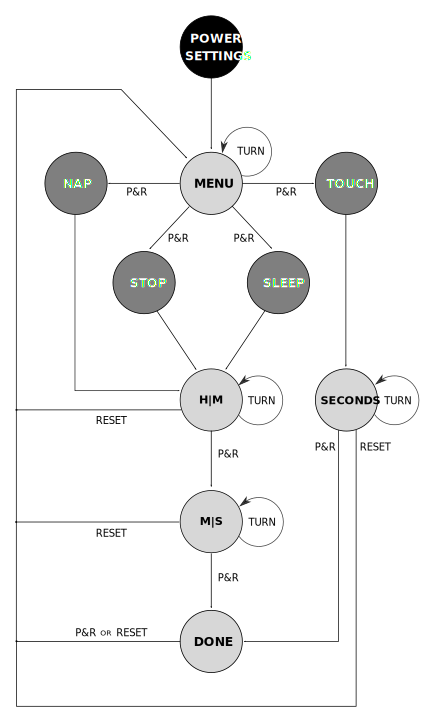
\includegraphics{images/power_settings_state_diagram.png}
  \caption{Power Settings - State Diagram}
\end{figure}
